%% source: 2023-sp-redemption_midterm_02
\begin{prob}
    A ``hub and spoke'' graph with $n$ nodes consists of a single ``hub'' node $h$
    along with $n - 1$ ``spoke'' nodes, $u_1, \ldots, u_{n-1}$ and $n - 1$
    edges from the hub node $h$ to each of the spoke nodes. For example, a ``hub and
    spoke'' graph with 8 nodes looks like the below:

    \begin{center} 
        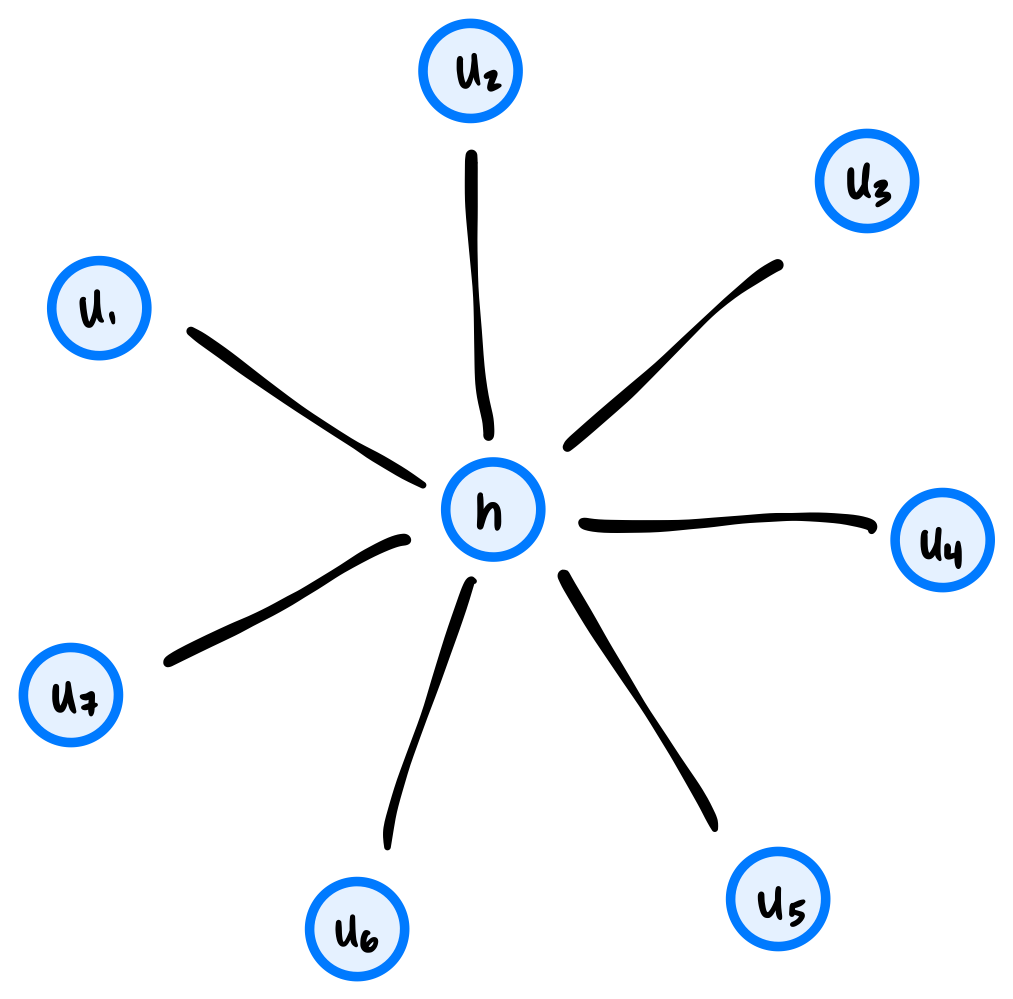
\includegraphics[width=.5\textwidth]{./fig/g5.png}
    \end{center}

    What is the \textbf{worst case} time complexity of an optimal algorithm
    which takes as input an arbitrary graph $G = (V, E)$ and determines if it
    is a ``hub and spoke'' graph? You may assume that the graph is represented as
    an adjacency list and that the total number of edges in the graph can be retrieved
    in constant time.

    \begin{choices}
        \correctchoice $\Theta(1)$
        \choice $\Theta(V)$
        \choice $\Theta(V + E)$
        \choice $\Theta(V^2)$
        \choice $\Theta(E^2)$
    \end{choices}

\end{prob}
